\documentclass{beamer}
\mode<presentation> {
%\usetheme{default}
\usetheme{AnnArbor}

%\usecolortheme{albatross}
\usecolortheme{beaver}
%\usecolortheme{beetle}
%\usecolortheme{crane}
%\usecolortheme{dolphin}
%\usecolortheme{dove}
%\usecolortheme{fly}
%\usecolortheme{lily}
%\usecolortheme{orchid}
%\usecolortheme{rose}
%\usecolortheme{seagull}
%\usecolortheme{seahorse}
%\usecolortheme{whale}
%\usecolortheme{wolverine}

%\setbeamertemplate{footline} % To remove the footer line in all slides uncomment this line
%\setbeamertemplate{footline}[page number] % To replace the footer line in all slides with a simple slide count uncomment this line

%\setbeamertemplate{navigation symbols}{} % To remove the navigation symbols from the bottom of all slides uncomment this line
}
\usepackage{graphicx} % Allows including images
\usepackage{booktabs} % Allows the use of \toprule, \midrule and \bottomrule in tables
%\usepackage[utf8]{inputenc}
\usepackage[english]{babel}
\usepackage{times}
%\linespread{1.5}
\usepackage{setspace}
\singlespacing 
\usepackage{soul}
\usepackage{amsmath}
\usepackage{enumitem}
\usepackage{mathrsfs}
\usepackage{amssymb}
\usepackage{amsthm}
\usepackage{multicol}
\usepackage{xr}
\usepackage{cancel}
\usepackage{graphicx}%
\usepackage{xfrac}
\usepackage{float}
%\usepackage[letterpaper, margin=1 in]{geometry}
\usepackage[rightcaption]{sidecap}
\usepackage{lipsum}                     
\usepackage{xargs}                      
%\usepackage[pdftex,dvipsnames]{xcolor} 
%\usepackage{color}
%white, black, red, green, blue, cyan, magenta, yellow
\usepackage{wrapfig}
\usepackage{epstopdf}
\epstopdfDeclareGraphicsRule{.pdf}{png}{.png}{convert #1 \OutputFile}
\DeclareGraphicsExtensions{.png,.pdf}
\graphicspath{ %{/home/rachellonchar/}{/home/rachellonchar/Pictures/}{media/rachellonchar/WINDOWS_USB/00 UMN Research and Classes/Fall 2017 Classes/}{/media/rachellonchar/WINDOWS_USB/00 UMN Research and Classes/Fall 2017 Classes}
{/home/rachellonchar/Dropbox/python_work/peat_project/g/net_inundation_aeration_periods/periods_as_MPPs/}, {/home/rachellonchar/Dropbox/python_work/peat_project/g/net_inundation_aeration_periods/}, {/home/rachellonchar/Dropbox/python_work/peat_project/g/} }
%defining comment functions
%\rnote{ } for Rachel notes
%\xnote{ } for Xue notes
\usepackage[colorinlistoftodos,prependcaption,textsize=small]{todonotes}
\newcommandx{\rnote}[2][1=]{\todo[inline, backgroundcolor=yellow!25, bordercolor=black, #1]{#2}}
%{\todo[disable,#1]{#2}} 
\newcommandx{\xnote}[2][1=]{\todo[inline, backgroundcolor=magenta!25, bordercolor=black, #1]{#2}}
%{\todo[disable,#1]{#2}}
%use to hide comments 

%----------------------------------------------------------------------------------------
%	TITLE PAGE
%----------------------------------------------------------------------------------------
\title[Peatland methane fluctuations]{Peatland methane emissions driven by interaction of soil temperature and water table 
} % The short title appears at the bottom of every slide, the full title is only on the title page
\author{Rachel Lonchar} 
\institute[UMN] % Your institution as it will appear on the bottom of every slide, may be shorthand to save space
{University of Minnesota \\ % Your institution for the title page
\medskip
\textit{lonch002@umn.edu} % Your email address
}
\date{\today} % Date, can be changed to a custom date
\begin{document}
%----------------------------------------------------------------------------------------
\begin{frame}
\titlepage % Print the title page as the first slide
\end{frame}
%----------------------------------------------------------------------------------------
\begin{frame}
\frametitle{Model Goal} % Table of contents slide, comment this block out to remove it
%FIG 3
We want to be able to express methane as a function of soil temperature and water table, e.g. 
\[CH_4 = f(T_{soil},WT) \]

We can further assume a different behavior based on whether soil is inundated or aerated. Namely, we could obtain the following model,
 \[
        CH_4=
\begin{cases}
f_1(T_{soil},WT), & \text{ inundated} \\
f_2(T_{soil},WT), & \text{ aerated} 
\end{cases}
  \]
where $f_1$, $f_2$ are more reasonably linear than $f$ alone is. 
\end{frame}
%----------------------------------------------------------------------------------------
%	PRESENTATION SLIDES
%----------------------------------------------------------------------------------------

%------------------------------------------------
\section{Motivation}
%------------------------------------------------
\begin{frame}
\frametitle{Motivation comes from prior research and Eddy covariance data from Bog Lake Fen.}
%Peatland carbon emissions previously linked to \textbf{soil temperature and water table} and Eddy covariance data from Bog Lake Fen demonstrate this link.%; extent of control is still uncertain 
%FIG 3
\begin{figure}[!htb]
\centering
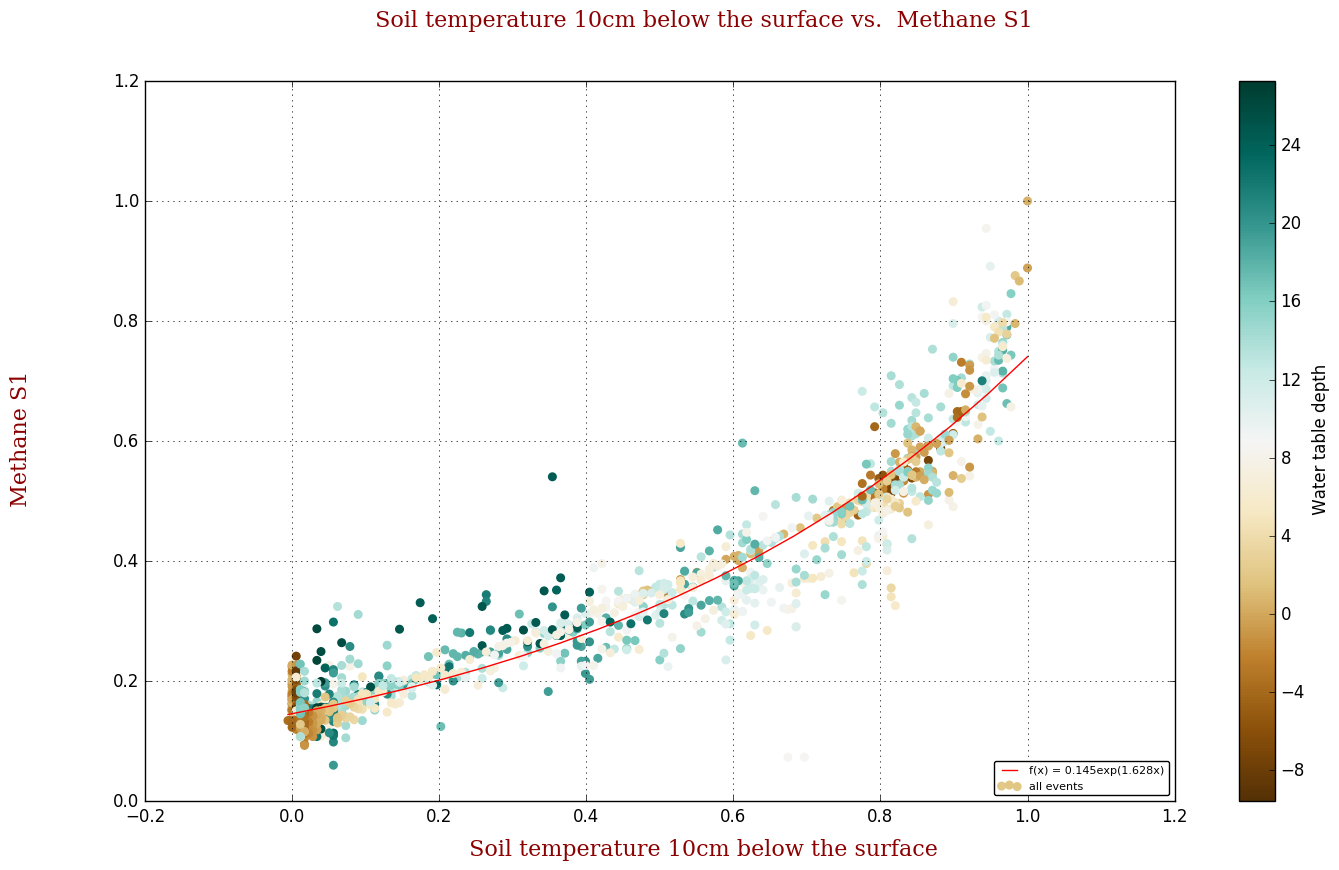
\includegraphics[width=.68\textwidth]{Ts10_vs_CH4_1518}
\caption{Methane can be modeled as a exponential function of soil temperature. Data here from open path measurements taken from 2015-2018.}
\end{figure}
~

\textbf{Hypotheses:}
 
1. Variations in methane release at constant temperatures indicate that soil temperature is not the only predictor of methane release. 

2. Water table is a secondary predictor of methane release.
\end{frame}

%
%%%%
\begin{frame}
Annual relationships deviate from the overall relationship between soil temperature and methane emissions, indicating there is something else at play.
\begin{figure}[!htb]
\centering
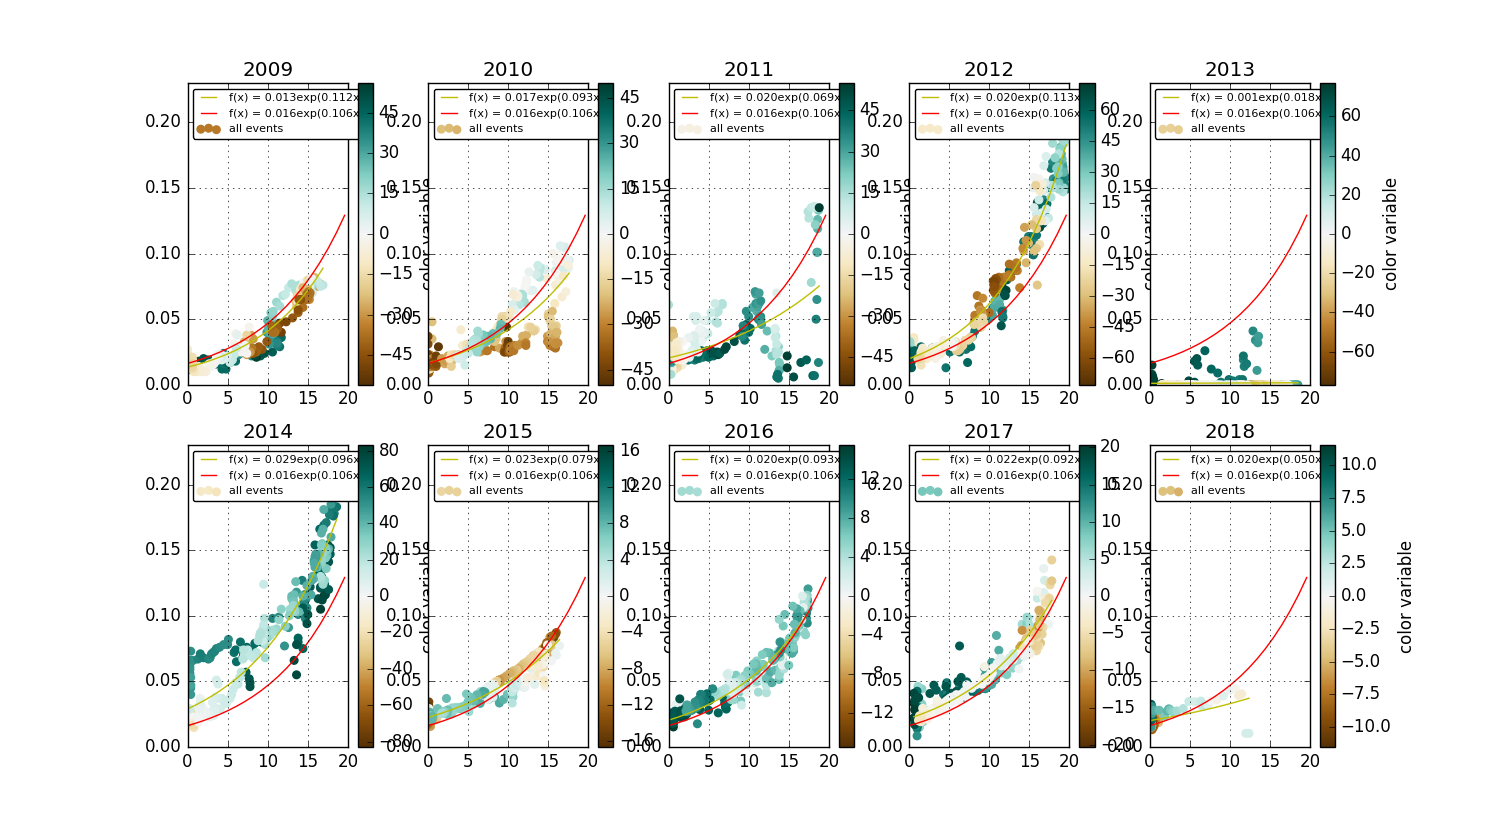
\includegraphics[width=\textwidth]{all_years_CH4_Ts}
\end{figure}
\end{frame}

\begin{frame}
Annual relationships deviate from the overall relationship between soil temperature and methane emissions, indicating there is something else at play.
\begin{figure}[!htb]
\centering
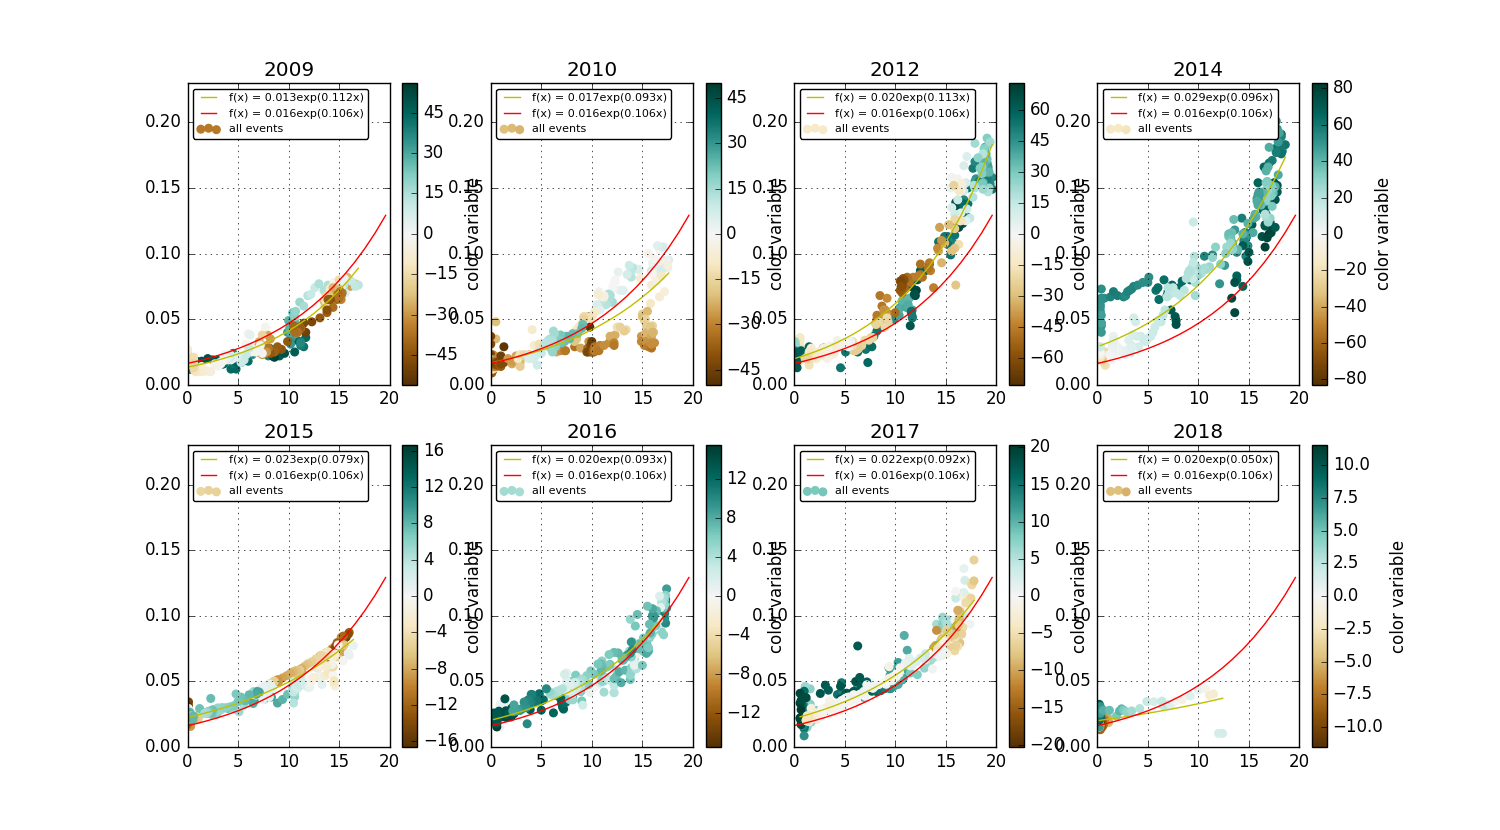
\includegraphics[width=\textwidth]{all_years_CH4_Ts_no1113}
\end{figure}
\end{frame}

\begin{frame}
Annual relationships deviate from the overall relationship between soil temperature and methane emissions, indicating there is something else at play.
\begin{figure}[!htb]
\centering
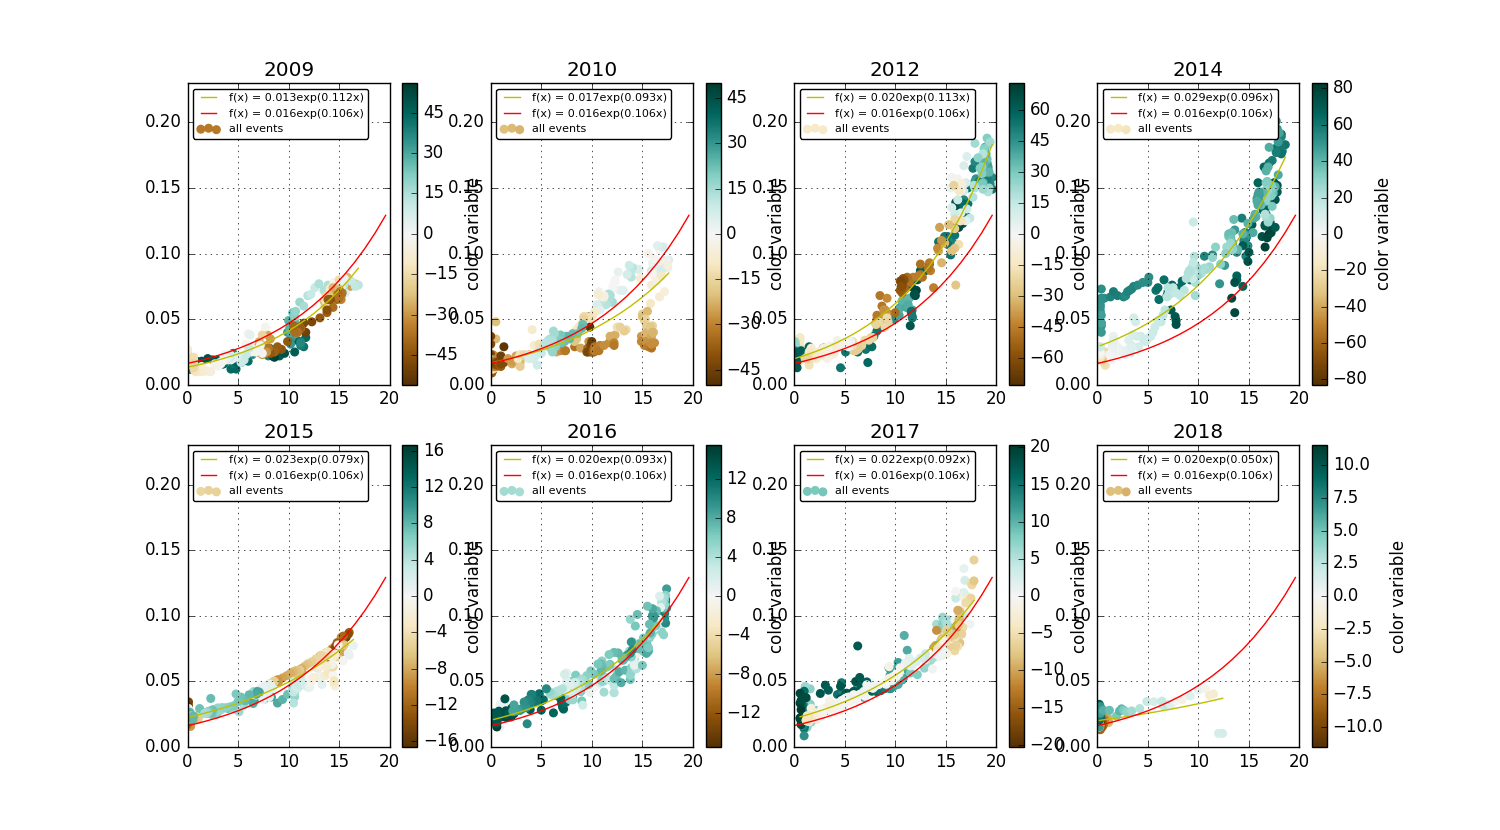
\includegraphics[width=\textwidth]{all_years_CH4_Ts_no1113}
\end{figure}
\end{frame}



\begin{frame}
\frametitle{Methane deviations are positively correlated with water table, and this relationship becomes stronger when we restrict ourselves to inundated events.}
\begin{figure}[!htb]
\centering
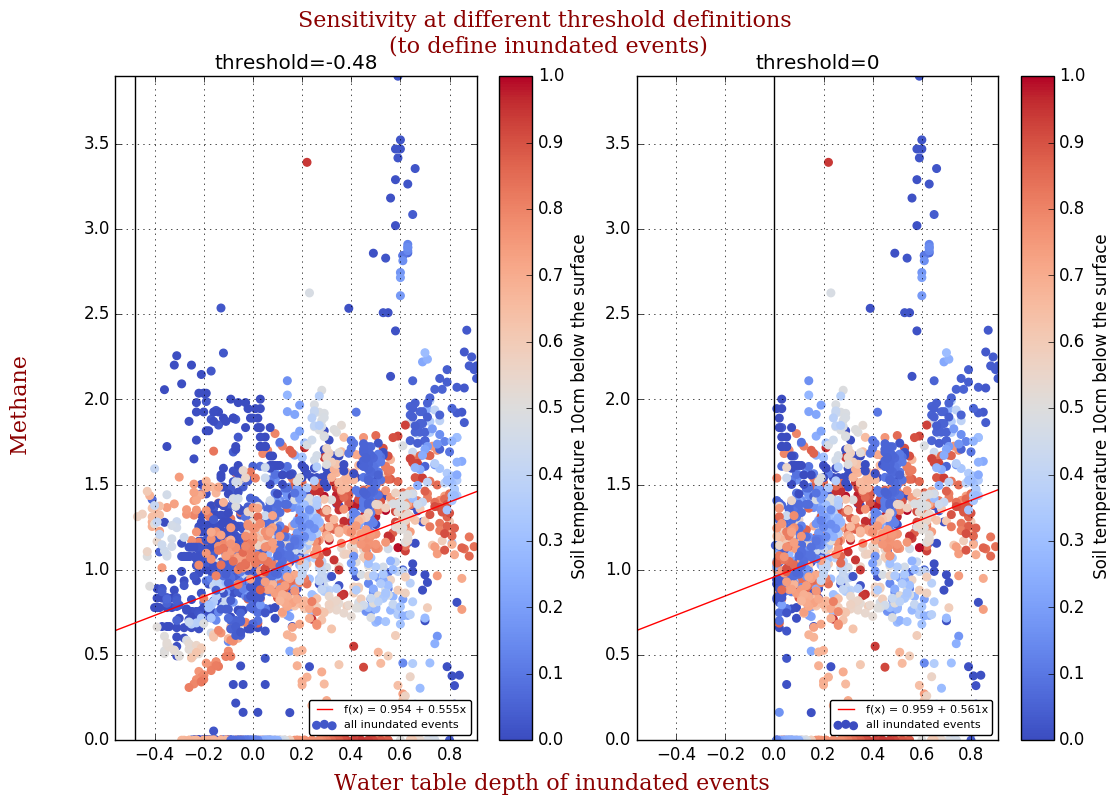
\includegraphics[width=.7\textwidth]{old_I2l}
\end{figure}
\end{frame}

\begin{frame}
\frametitle{Methane deviations are positively correlated with water table, but this relationship becomes \textit{negative} when we restrict ourselves to aerated events. }
\begin{figure}[!htb]
\centering
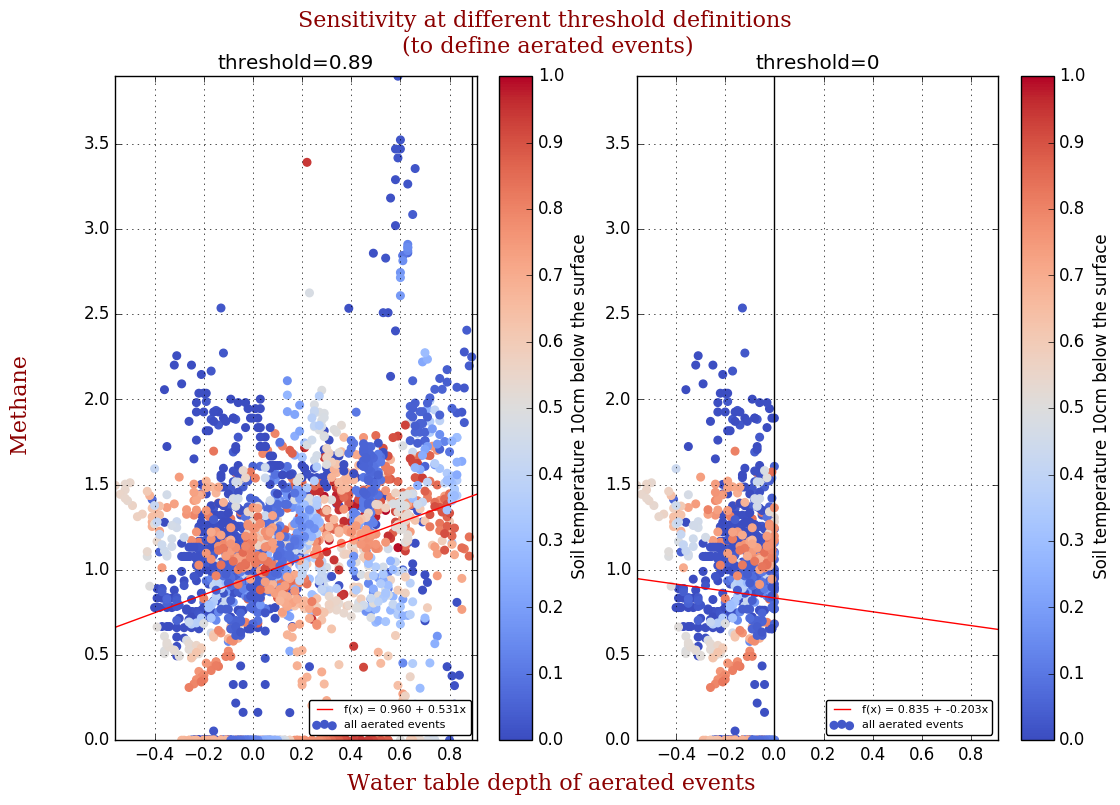
\includegraphics[width=.7\textwidth]{old_A2l}
\end{figure}
\end{frame}

\begin{frame}
\frametitle{Methane's sensitivity to water table is dependent on the state of the system, e.g. whether or not the peat is inundated or aerated.}
Considerations:
\\
Biological mechanism?
\\
Transport and production of methane are separate processes that both depend on water table.
\\~\\
Looking forward: Dichotomous Markov process?

\end{frame}

%------------------------------------------------
%References 
%------------------------------------------------


%------------------------------------------------
\section{Citations} 
\begin{frame}
%\frametitle{References}
\begin{thebibliography}{9}
\footnotesize{
\bibitem{aselmann}
Aselmann, I., P. J. Crutzen. \textit{Atmos Chem} \textbf{8}, 307-358, 1989.

\bibitem{Holden}
Holden, J.
\textit{Phil. Trans. R. Soc. A}, \textbf{363}, 2891-2913, 2005.

\bibitem{MEF}
Kolka, R., S. Sebestyen, E. Verry, and K. Brooks. \textit{Peatland Biogeochemistry and Watershed Hydrology at the  Marcell Experimental Forest}.
CRC Press,
2011. %https://www.nrs.fs.fed.us/EF/Marcell/data/

\bibitem{Laio}
Laio, F., S. Tamea, L. Ridolfi, P. D'Odorico, I. Rodriguez-Iturbe.
\textit{Water Resources Research}, \textbf{45}, W05419, 2009.

\bibitem{fung}
Matthews, E., I. Fung. \textit{Glob. Biogeochem. Cycles}, \textbf{1}, 61-86, 1987.

\bibitem{eco_text}
Rodriguez-Iturbe, I., A. Porporato, L. Ridolfi, V. Isham, D. R. Cox.
\textit{Proc. R. Soc. Lond. A}, \textbf{455}, 3789-3805, 1999.
}
\end{thebibliography}
%\endgroup
\end{frame}
%------------------------------------------------

%----------------------------------------------------------------------------------------

\end{document} 